% !TEX encoding = UTF-8 Unicode
\chapter{Tratamiento de datos y resultados} 

Durante el desarrollo de este capítulo se analizarán los resultados obtenidos al aplicar las técnicas anteriormente mencionadas a los datos recopilados.

\section{Caracterización de los eventos}

En primer lugar se decidió construir las gráficas correspondientes a las señales adquiridas por el acelerómetro durante los recorridos.
Se resaltan en diferentes colores las señales correspondientes a cada evento detectable: rojo para el evento de frenado, verde para el evento de rebase y magenta para el evento de movimiento en zig-zag. 
Los datos relativos al modo de conducción normal se encuentran en color azul. 

A continuación se presentan las gráficas correspondientes a la aceleración registrada con respecto al tiempo transcurrido en los recorridos. 
Cada gráfica contiene información de uno de los tres ejes sobre los que se encontraba alineado el sensor.

Las unidades de aceleración en el eje $y$ de las gráficas corresponden a un formato específico que maneja el sensor utilizado; si se desean conocer las cantidades correspondientes en $m/s^2$ basta con aplicar la siguiente conversión; donde $x$ es la aceleración manejada por el sensor y $a$ es el valor de la misma en $m/s^2$.\\

$$a={9.81\over 25.5}(x-127)$$

\ \\

esta ecuación fue determinada al calibrar el sensor.\\

La gráfica de la señal obtenida en la prueba del vehículo estático muestra un comportamiento oscilatorio, de amplitud relativamente pequeña en comparación con los cambios de aceleración manejados en los recorridos, cuyos valores máximos son cercanos a $g$ (el valor correspondiente a $g$ en el formato del sensor es aproximadamente 25.5 unidades).
Únicamente se presenta la señal obtenida sobre el eje $z$ (figura \ref{1z2.pdf}) debido a que es el eje sobre el cual se registra la aceleración debida a la vibración del motor, además de que las señales de los ejes restantes tienen una forma similar\zsavepos{similar}.
\vspace{12.2cm}
\graficaceroeventos{1z2.pdf}{Vehículo estático}{z}{\dimexpr\paperheight-\zposy{similar}sp+10mm}

Al analizar los resultados de esta prueba se concluyó que la contribución al ruido en la señal por parte del motor y otros factores externos era irrelevante; ya que, tanto en la prueba del vehículo estático como en una situación en donde el acelerómetro permanece inmóvil en una superficie plana, se obtienen señales cuya amplitud, en promedio, no varía significativamente de una prueba a otra.
Por lo cual la oscilación de esta señal es principalmente debida al ruido blanco inherente al sensor; y debido a ello, el ruido provocado por los factores mencionados se considera como despreciable.
De no ser así, la vibración del motor provocaría que la amplitud promedio de la señal obtenida fuese mayor que la obtenida al dejar el sensor sobre una superficie inmóvil.

Los registros de aceleración de la prueba de conducción regular (figuras \ref{2x.pdf}, \ref{2y.pdf} y \ref{2z.pdf}) no presentan, como se esperaba, ninguna anomalía importante, exceptuando la cresta presente en los datos registrados en el eje $y$ del sensor, la cual es debida a la aceleración centrípeta generada al recorrer una curva.
\pagebreak

\ \\
\vspace{27cm}
\graficaceroeventos{2x.pdf}{Conducción regular}{x}{40mm}
\graficaceroeventos{2y.pdf}{Conducción regular}{y}{147mm}
\pagebreak
\ \\
\vspace{10.4cm}
\graficaceroeventos{2z.pdf}{Conducción regular}{z}{40mm}

Durante el recorrido destinado para el evento de frenado se obtuvieron los siguientes registros (figuras \ref{3x.pdf}, \ref{3y.pdf} y \ref{3z.pdf}):
\pagebreak

\ \\
\vspace{27cm}
\graficauneventos{3x.pdf}{Frenado}{x}{40mm}
\graficauneventos{3y.pdf}{Frenado}{y}{147mm}
\pagebreak
\ \\
\vspace{10.4cm}
\graficauneventos{3z.pdf}{Frenado}{z}{40mm}

Como se puede observar en la gráfica correspondiente al eje $x$, la notoriedad del evento en esta dimensión es evidente; consiste en una disminución drástica de la aceleración durante los instantes en que se frena al vehículo, seguido de un aumento de esta. 
Tal aumento de aceleración concuerda con lo mencionado en la descripción del evento.
Sobre los ejes $y$ y $z$ no se aprecia ningún cambio considerable en los intervalos donde ocurren los eventos.
Las anomalías que se presentan durante algunos de los periodos de conducción regular (principalmente en el eje $y$) son debidas a la ya mencionada aceleración centrípeta al recorrer una curva.  
Otra de las causas de estas anomalías son los movimientos característicos del vehículo cuando este se incorpora al carril de tránsito, estando ubicado inicialmente a un lado de este y partiendo de un estado de reposo.\\

En el recorrido dedicado al evento de rebase se obtuvo lo siguiente (figuras \ref{4x.pdf}, \ref{4y.pdf} y \ref{4z.pdf}):

\pagebreak
\ \\
\vspace{27cm}
\graficauneventos{4x.pdf}{Rebase}{x}{40mm}
\graficauneventos{4y.pdf}{Rebase}{y}{147mm}
\pagebreak
\ \\
\vspace{10.4cm}
\graficauneventos{4z.pdf}{Rebase}{z}{40mm}

En el caso del evento de rebase, el evento no destaca mucho visualmente como lo hace el evento de frenado, pero si lo suficiente como para identificarlo a simple vista en la gráfica correspondiente al eje $x$. 
Se puede observar que el evento consiste en un aumento de la aceleración, lo cual es consistente con el evento de rebase. 
Se esperaba obtener también características discriminantes para este evento en el eje $y$, debido a la aceleración transmitida sobre esa dirección al cambiar de carril. 
Sin embargo, a simple vista no parece haber nada destacable, lo cual se atribuye a que la aceleración en esa dirección no posee la magnitud suficiente para generar una característica discriminable en la gráfica.\\

Las gráficas relacionadas a el evento de movimiento en zig-zag se presentan a continuación (figuras \ref{5x.pdf}, \ref{5y.pdf} y \ref{5z.pdf}):

\pagebreak
\ \\
\vspace{27cm}
\graficadoseventos{5x.pdf}{Movimiento en zig-zag}{Rebase}{x}{40mm}
\graficadoseventos{5y.pdf}{Movimiento en zig-zag}{Rebase}{y}{147mm}
\pagebreak
\ \\
\vspace{10.4cm}
\graficadoseventos{5z.pdf}{Movimiento en zig-zag}{Rebase}{z}{40mm}

El evento de movimiento en zig-zag es gráficamente el más notable de los tres. 
Se aprecia claramente, sobre el eje $y$, la aceleración característica del ir y venir del vehículo, con una amplitud muy notoria en las oscilaciones. 
Por otro lado, sobre el eje $x$, es el evento de rebase es el que ahora toma relevancia, tal y como en las gráficas correspondientes al recorrido dedicado a este evento.

Debido a que la teoría con la que se tenía pensado trabajar requiere que la frecuencia de muestreo de la señal a analizar sea siempre la misma, se optó por realizar una interpolación a los datos obtenidos en los recorridos. 
Ya que, si bien en periodos de tiempo largos los dispositivos de medición arrojaban la cantidad de datos correspondiente a su frecuencia de muestreo, al revisar los intervalos de tiempo entre datos consecutivos, se observó que estos intervalos difícilmente eran los mismos. 
Debido a esto se elaboró un programa para interpolar linealmente puntos que estuvieran separados entre sí la misma cantidad de tiempo, con lo cual se resolvería el problema de la separación de los datos.

Después de realizar la interpolación se procedió a analizar los conjuntos de datos de cada recorrido mediante {\em ventanas de análisis} de $15s$ de duración, desplazadas a intervalos de $0.5s$. 
Lo cual consistió en tomar los datos registrados desde $0$ hasta $15s$ sobre cada uno de los tres ejes en un cierto recorrido, para luego obtener el espectro de frecuencias de cada una de las tres series. 
Después, ya que el intervalo de separación entre una ventana y la siguiente era de $0.5s$, se tomaba el siguiente conjunto de datos sobre cada eje, el cual iba desde $0.5$ hasta $15.5s$. Posteriormente se obtenían los espectros correspondientes y se continuaba con el siguiente conjunto, el cual iba de $1$ a $16s$. 
Este proceso continua hasta llegar al conjunto cuyo intervalo de tiempo va desde $T-15s$ hasta $T$, siendo $T$ el tiempo total del recorrido en cuestión (si $T$ no fuese múltiplo de $0.5$, este se sustituía por el múltiplo anterior más cercano).
Cabe mencionar que para cada serie de tiempo contenida en una ventana existen dos espectros de frecuencias calculados; uno relativo a las amplitudes y frecuencias de las funciones seno; y otro igualmente relacionado a las amplitudes y frecuencias de las funciones coseno.
Debido a que las características de los espectros relativos a cada función obtenidos son muy similares, se hará referencia de forma generalizada a espectros y frecuencias, sin distinguir a qué tipo de función pertenecen a menos que se considere necesario. 

Una vez obtenidos los espectros de todas las ventanas sobre los tres ejes, estos se analizaron uno por uno, con el objetivo de identificar las frecuencias que llegasen a tener las amplitudes de mayor magnitud durante cada recorrido analizado.
Lo anterior se realizó con la ayuda de un algoritmo implementado por un programa de computadora, cuya labor era registrar en un documento cualquier amplitud cuyo valor absoluto fuese mayor a un umbral definido; documento en el cual, además de la amplitud, también se anotaban el tiempo y el eje correspondientes al espectro en cuestión, así como la frecuencia relativa a tal amplitud.
Luego de que se filtrarán las frecuencias de cada una de las ventanas de un recorrido se analizaban los resultados obtenidos; con el fin de determinar las frecuencias que estuviesen relacionadas con los eventos realizados. 
Se eligieron como {\em frecuencias características} las que tuviesen una mayor amplitud en los periodos de tiempo relativos a la realización de los eventos que se deseaban detectar. 
Ya que, muy probablemente serían estas las frecuencias que tendrían una mayor contribución a la forma característica de cada evento en las gráficas.
Dichas frecuencias se dan a conocer en la tabla \ref{tablasfrec}.\\

\begin{table}[H]
\centering
\begin{tabular}{c|c|c}
\hline \hline
\bf Evento &\bf Frecuencias características & \bf Eje \\ 
\hline \hline
\multirow{2}{*}{Frenado} & $0.066Hz$ & \multirow{4}{*}{$x$} \\ \cline{2-2}
& $0.133Hz$ & \\ \cline{1-2}
\multirow{2}{*}{Rebase} & $0.066Hz$ & \\ \cline{2-2}
& $0.133Hz$ & \\ \hline
Zig-zag & $0.266Hz$ & $y$\\
\hline \hline
\end{tabular}
\caption{Frecuencias características de cada evento.}
\label{tablasfrec}
\end{table}

A continuación se muestran ejemplos de tres espectros de frecuencias (figuras \ref{Espectro_fxs.pdf}, \ref{Espectro_rxs.pdf} y \ref{Espectro_zyc.pdf}), uno para cada tipo de evento, sobre el eje de interés donde sus frecuencias características son relevantes. 
Cada uno de ellos fueron calculados a partir de una serie de tiempo contenida en una ventana, en la cual se encontraban los datos relativos a la ejecución del evento en cuestión. Se trabajó únicamente con los valores absolutos de las amplitudes durante el análisis.

\pagebreak
\ \\
\vspace{27cm}
\graficaespectros{Espectro_fxs.pdf}{Frenado}{x}{40mm}{Frecuencias 
características}
\graficaespectros{Espectro_rxs.pdf}{Rebase}{y}{147mm}{Frecuencias características}  
\pagebreak
\ \\
\vspace{10.4cm}
\graficaespectros{Espectro_zyc.pdf}{Movimiento en zig-zag}{y}{40mm}{Frecuencia característica}

Después de determinar las frecuencias características de cada evento (marcadas en color azul), el siguiente paso sería aplicar un criterio de detección efectivo, con base en las ventanas de tiempo descritas anteriormente. 
Dicho método está basado en las amplitudes que tienen las frecuencias características de los eventos a lo largo del tiempo que dura cada recorrido.

La técnica usada para la detección de los eventos es la separación de grupos por el método de redes neuronales. 
En la cuál, mediante un programa de computadora, se introduce en un algoritmo un vector de tres componentes, el cual contiene en cada una de ellas un número real cualquiera. 
Cada componente corresponde a alguna de las tres frecuencias características de los eventos ($0.066Hz$ y $0.133Hz$ para los eventos de frenado y rebase, y $0.266Hz$ para el evento de zig-zag), y su valor representa la amplitud de la función armónica (seno o coseno) de tal frecuencia. 
Si estas amplitudes están dentro del rango de las que caracterizan a los eventos detectables, entonces la salida del algoritmo será otro vector, característico del evento en cuestión. 
Si la entrada no corresponde a ninguno de los eventos, la salida obtenida será un vector característico de esta situación (cuyas componentes usualmente son valores cercanos a cero).
Las salidas características de cada evento se muestran en la tabla \ref{tablasalidas}.\\

\begin{table}[H]
\centering
\begin{tabular}{c|c|c|c}
\hline \hline
\bf Evento &\bf Componente 1 &\bf Componente 2 &\bf Componente 3\\ 
\hline \hline
Frenado & $\approx 1$ & $\approx 0$ & $\approx 0$ \\ 
Rebase & $\approx 0$ & $\approx 1$ & $\approx 0$ \\ 
Zig-zag & $\approx 0$ & $\approx 0$ & $\approx 1$ \\
\hline \hline
\end{tabular}
\caption{Salidas características de cada evento (los valores que cada salida puede tomar van de $0$ a $1$).}
\label{tablasalidas}
\end{table}

En la práctica, para que el algoritmo reconozca un valor como {\em aproximadamente} $1$ o {\em aproximadamente} $0$, se deben establecer ciertos {\em valores frontera}, por encima o por debajo de los cuales a un número se le asigna alguna de estas propiedades.
En este caso en particular se estableció que un número es aproximadamente $1$ cuando es mayor o igual a $0.7$; mientras que se considera aproximadamente $0$ cuando es menor o igual a $0.3$.

Si las salidas del algoritmo no corresponden a ningún evento, se considera que se realizó una conducción regular.

De esta manera, al introducir el vector de amplitudes cada $0.5s$, el cual es el tiempo de separación entre los espectros calculados para cada ventana, se puede saber, si en los $15s$ (o menos) anteriores el vehículo realizó o no cualquiera de los tres eventos.

Debido a que los vectores de entrada poseen tres componentes, estos se pueden interpretar como puntos en un espacio de tres dimensiones.
Se elaboró una gráfica con la información de las frecuencias características para algunas de las ventanas que contenían registros de los eventos realizados y de conducciones regulares, la cual se presenta a continuación.
\pagebreak

\begin{figure}[H]
\centering
\vspace{8.5cm}
\begin{textblock*}{\textwidth}(1.5cm,3cm)
\begin{tikzpicture}
  \node at (-8,0) {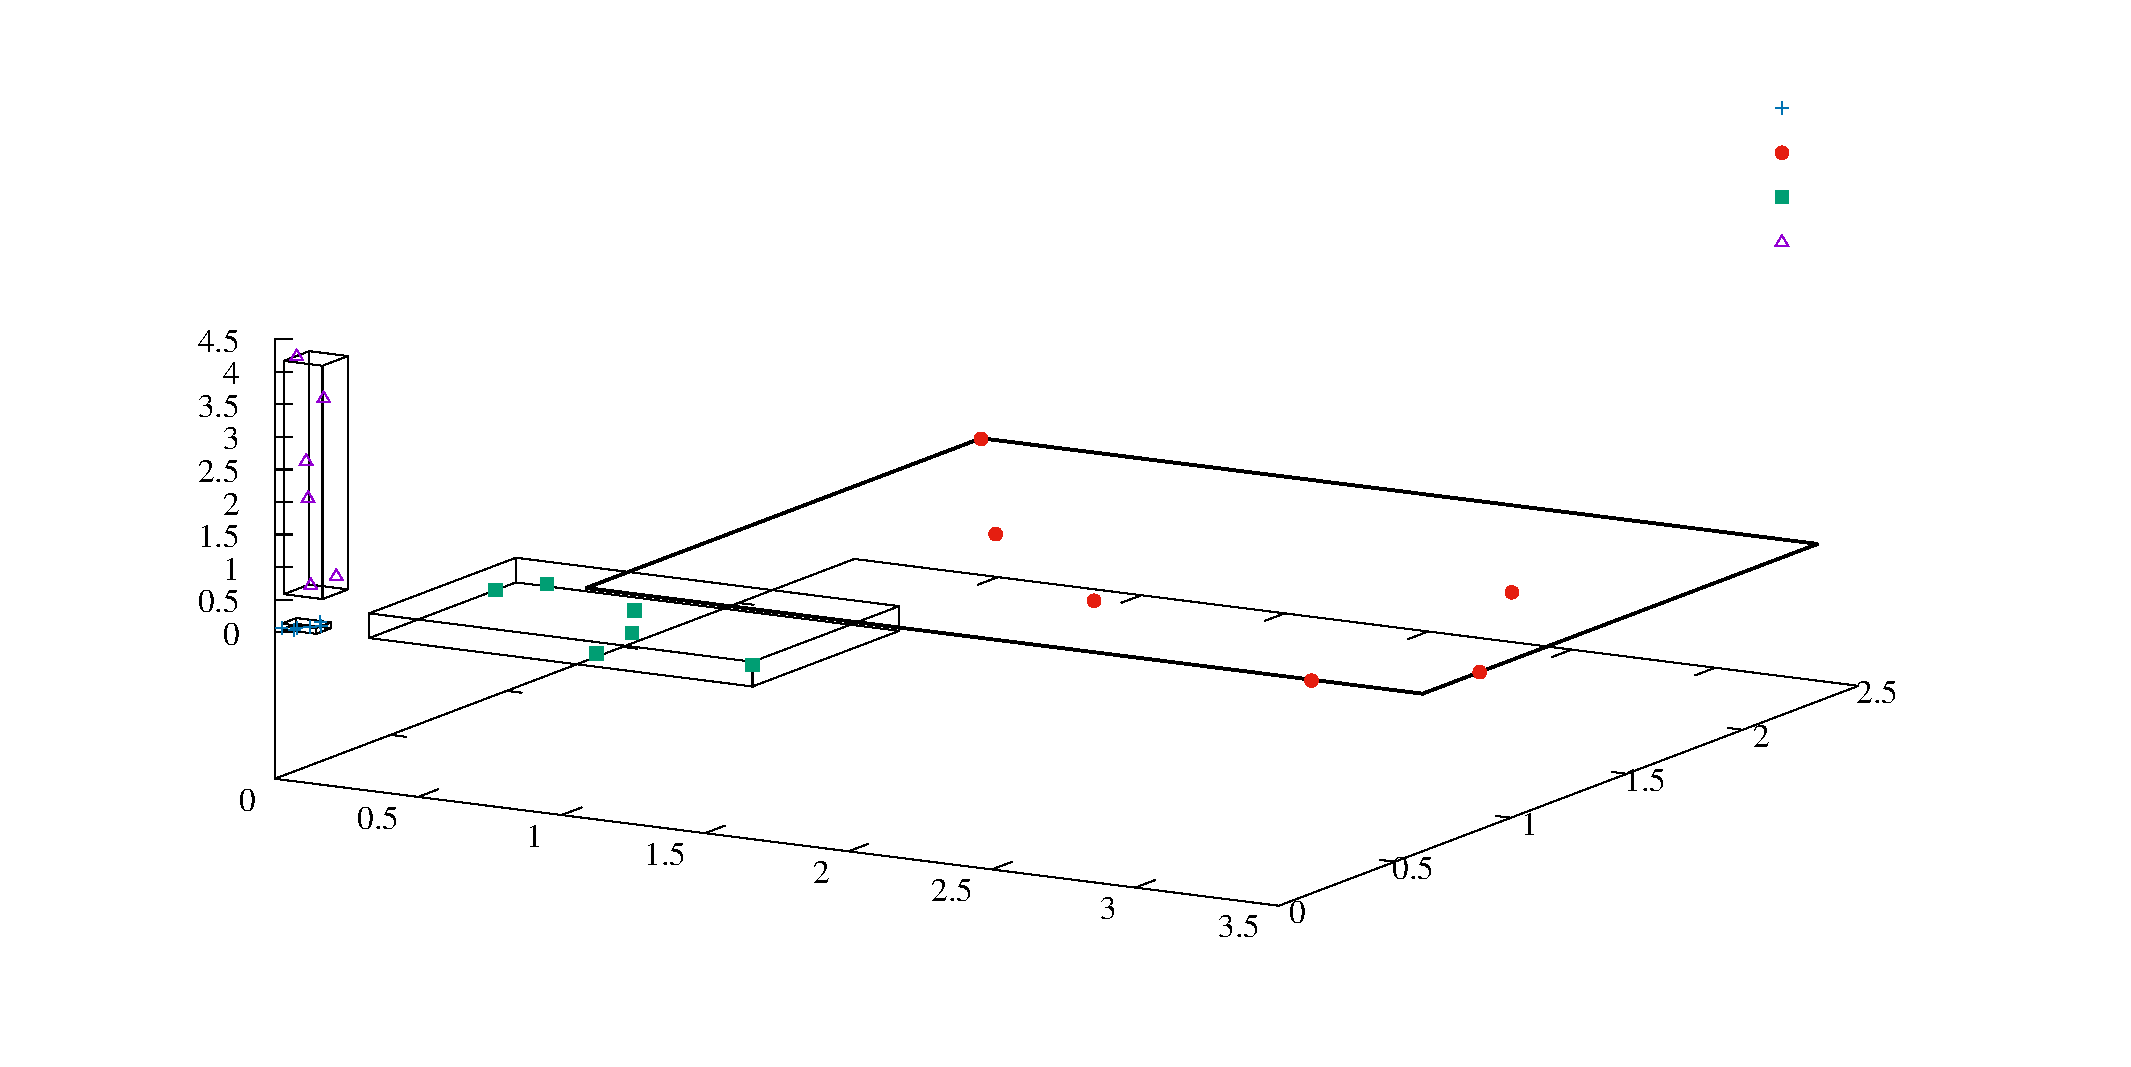
\includegraphics[scale=0.55]{Cajas.pdf}};
  \node at (-8.3,3) {\bf Regiones características de cada evento};
  \node[rotate=353] at (-11,-3.7) {Amplitud (0.066 Hz)};
  \node[rotate=20] at (-2.6,-3) {Amplitud (0.133 Hz)};
  \node[rotate=90] at (-16.4,-.5) {Amplitud (0.266 Hz)};
  \node at (-2,4) {\fontsize{8}{1}\selectfont Regular};
  \node at (-2.03,3.57) {\fontsize{8}{1}\selectfont Frenado};
  \node at (-2.01,3.15) {\fontsize{8}{1}\selectfont Rebase};
  \node at (-2,2.73) {\fontsize{8}{1}\selectfont Zig-zag};
\end{tikzpicture}
\end{textblock*}
\caption{Cada eje contiene los valores de las amplitudes para una de las tres frecuencias características.}
\label{Cajas}
\end{figure}

En la figura \ref{Cajas} se puede apreciar claramente la tendencia de los puntos de un mismo evento a agruparse en una determinada región.
Cada eje del espacio tridimensional corresponde a una de las frecuencias características de los eventos. 
Mientras que las coordenadas de cada eje representan la amplitud relativa a cada frecuencia. 
Según el valor de estas amplitudes, el punto en cuestión puede o no pertenecer a alguno de los eventos. 
Como se aprecia en la imagen existen diferentes zonas con forma de prisma, cada una de las cuales contiene puntos de determinado evento o de conducción regular. 
Dichos prismas dan una idea del espacio donde los valores de las amplitudes para un punto entran en la categoría de alguno de los tres eventos o de una conducción regular.
Estos prismas corresponden a las medidas de incertidumbre asociadas a cada una de las clases. 
Cada punto de la gráfica fue obtenido del espectro de frecuencias de ventanas que contenían muestras de datos de los eventos y conducciones regulares realizados.

Al hacer pasar la ventana de tiempo a la señal completa de un recorrido, se obtienen decenas de puntos como los de la figura \ref{Cajas}. 
Estos puntos se introducen como entrada del algoritmo antes mencionado, el cual como se mencionó consiste principalmente en una red neuronal que determina a qué tipo de evento pertenece la información de entrada.
Debido a que se usaron las funciones seno y coseno como funciones base para implementar la transformada de Fourier, existen dos puntos con información de frecuencias características para cada ventana de tiempo; uno relativo a las funciones seno y otro a las funciones coseno.
Por lo cual, se implementó el algoritmo de detección en tres modalidades distintas: en una se empleó la información de las frecuencias características relativas a las funciones coseno, en otra se hizo lo mismo con la información de las funciones seno, y en una tercera modalidad se intentó mejorar los resultados de detección de las dos anteriores, al establecer una función que utilice la información de las dos funciones armónicas.
Esta última modalidad solo consiste en multiplicar las componentes de la misma frecuencia de las salidas relativas a cada función armónica; con lo cual se genera un nuevo vector de salida al asignar cada uno de los tres productos a su componente correspondiente.
Este nuevo vector es el que se utiliza como salida para dicha modalidad.
Los resultados de la implementación de las tres modalidades del algoritmo se muestran a continuación (figuras de \ref{Deteccion_3_C.pdf} a \ref{Deteccion_5_CxS.pdf}):

\pagebreak
\ \\
\vspace{27cm}
\graficadeteccion{Deteccion_3_C.pdf}{de frenado}{cosenos}{Regular}{Rebase}{Zig-zag}{Frenado}{40mm}
\graficadeteccion{Deteccion_3_S.pdf}{de frenado}{senos}{Rebase}{Regular}{Zig-zag}{Frenado}{147mm}
\pagebreak
\ \\
\vspace{10.4cm}
\graficadeteccion{Deteccion_3_CxS.pdf}{de frenado}{producto de salidas}{Regular}{Rebase}{Frenado}{}{40mm}

\pagebreak
\ \\
\vspace{27cm}
\graficadeteccion{Deteccion_4_C.pdf}{de rebase}{cosenos}{Rebase}{Regular}{}{}{40mm}
\graficadeteccion{Deteccion_4_S.pdf}{de rebase}{senos}{Rebase}{Regular}{Zig-zag}{}{147mm}
\pagebreak
\ \\
\vspace{10.4cm}
\graficadeteccion{Deteccion_4_CxS.pdf}{de rebase}{producto de salidas}{Rebase}{Regular}{}{}{40mm}

\pagebreak
\ \\
\vspace{27cm}
\graficadeteccion{Deteccion_5_C.pdf}{de movimiento en zig-zag}{cosenos}{Rebase}{Regular}{Zig-zag}{}{40mm}
\graficadeteccion{Deteccion_5_S.pdf}{de movimiento en zig-zag}{senos}{Rebase}{Regular}{Zig-zag}{}{147mm}
\pagebreak
\ \\
\vspace{10.4cm}
\graficadeteccion{Deteccion_5_CxS.pdf}{de movimiento en zig-zag}{producto de salidas}{Rebase}{Regular}{Zig-zag}{}{40mm}

Después de analizar los resultados de detección de las tres modalidades, se decidió utilizar la tercera modalidad como parte del método de detección empleado para el último recorrido. 
Se realizó dicha elección debido a que, es la modalidad que presenta menor cantidad de errores en la detección de eventos anómalos y de conducciones regulares.

Complementariamente se presentan las gráficas de los valores de cada componente del vector de salida del algoritmo para cada ventana de tiempo (figuras de \ref{Salidas_3_C.pdf} a \ref{Salidas_5_CxS.pdf}).
Dichos valores concuerdan con las gráficas de detección.

\pagebreak
\ \\
\vspace{27cm}
\graficasalidas{Salidas_3_C.pdf}{Frenado}{Componente 1}{Componente 2}{Componente 3}{cosenos}{40mm}
\graficasalidas{Salidas_3_S.pdf}{Frenado}{Componente 1}{Componente 2}{Componente 3}{senos}{147mm}
\pagebreak
\ \\
\vspace{10.4cm}
\graficasalidas{Salidas_3_CxS.pdf}{Frenado}{Componente 1}{Componente 2}{Componente 3}{producto de salidas}{40mm}

\pagebreak
\ \\
\vspace{27cm}
\graficasalidas{Salidas_4_C.pdf}{Rebase}{Componente 1}{Componente 2}{Componente 3}{cosenos}{40mm}
\graficasalidas{Salidas_4_S.pdf}{Rebase}{Componente 1}{Componente 2}{Componente 3}{senos}{147mm}
\pagebreak
\ \\
\vspace{10.4cm}
\graficasalidas{Salidas_4_CxS.pdf}{Rebase}{Componente 1}{Componente 2}{Componente 3}{producto de salidas}{40mm}

\pagebreak
\ \\
\vspace{27cm}
\graficasalidas{Salidas_5_C.pdf}{Zig-zag}{Componente 1}{Componente 2}{Componente 3}{cosenos}{40mm}
\graficasalidas{Salidas_5_S.pdf}{Zig-zag}{Componente 1}{Componente 2}{Componente 3}{senos}{147mm}
\pagebreak
\ \\
\vspace{10.4cm}
\graficasalidas{Salidas_5_CxS.pdf}{Zig-zag}{Componente 1}{Componente 2}{Componente 3}{producto de salidas}{40mm}

\pagebreak

\section{Validación de la propuesta}

El último recorrido se realizó con la intención de validar los métodos de detección implementados en la sección anterior; motivo por lo cual, este recorrido no fue involucrado en la obtención de frecuencias características, ni ningún otro proceso de análisis; únicamente fue utilizado con fines de detección.
Durante el trayecto se ejecutaron los tres diferentes tipos de eventos, obteniendo los siguientes registros (figuras \ref{6x.pdf}, \ref{6y.pdf} y \ref{6z.pdf}):\zsavepos{registros}

\vspace{12.2cm}
\graficatreseventos{6x.pdf}{Recorrido para validación}{Zig-zag}{Frenado}{Rebase}{x}{\dimexpr\paperheight-\zposy{registros}sp+30mm}
\pagebreak
\ \\
\vspace{27cm}
\graficatreseventos{6y.pdf}{Recorrido para validación}{Zig-zag}{Frenado}{Rebase}{y}{40mm}
\graficatreseventos{6z.pdf}{Recorrido para validación}{Zig-zag}{Frenado}{Rebase}{z}{147mm}
\pagebreak

Observando la gráfica relacionada al eje $x$, se puede apreciar fácilmente el patrón característico del evento de frenado y con una amplitud menor, el pico generado por el evento de rebase. 
Como se ha visto anteriormente, el evento de frenado y rebase no tienen mucha relevancia sobre el eje $y$.
El evento de movimiento en zig-zag, al igual que en las demás gráficas del eje $x$ donde está presente, no tiene mucha notoriedad en esta dimensión, no así en el eje $y$, donde es el evento que se puede identificar con mayor facilidad. 
Por último, en lo que corresponde al eje $z$, ninguno de los eventos es diferenciable a simple vista de los demás.

De los resultados de detección obtenidos en la sección anterior para la tercera modalidad, se observó que, en la mayoría de los casos, en los primeros segundos de la realización de cada evento el algoritmo, este no es capaz de reconocer el evento en cuestión con un grado de eficiencia aceptable.
Esto es debido a que, en los primeros segundos de la realización de un evento, la ventana no contiene suficientes datos del evento para que en su espectro se obtengan valores relevantes, correspondientes a las frecuencias características.
Como consecuencia de esto, se obtiene una combinación de detección del eventos anómalos junto con varias detecciones de conducción regular; lo cual baja considerablemente la eficiencia en la detección.

Existen varios métodos para mejorar la detección durante el periodo mencionado, sin embargo, tales métodos requieren de herramientas teóricas de diferente temática a las aquí utilizadas; la forma implementar el algoritmo de detección al presente recorrido de validación se describe a continuación.

La ventana de detección recorre los intervalos etiquetados como conducción regular de principio a fin.
La eficiencia en la detección de una conducción regular se calcula dividiendo el número de veces que el algoritmo detectó una conducción regular en los intervalos de tiempo con esta etiqueta, entre el número total de ventanas presentes en dichos intervalos.

Para cualquiera de los tres eventos detectables, la ventana inicia su recorrido cinco segundos después de comenzar el evento y lo termina cuando el evento finaliza, por lo que se anula la detección durante los primeros cinco segundos a partir del inicio de un evento.
La eficiencia en la detección de los eventos se calcula de forma análoga a la de la conducción regular.

Los resultados de detección para este recorrido se presentan en las siguientes gráficas (figuras \ref{Deteccion_6_C.pdf}, \ref{Deteccion_6_S.pdf} y \ref{Deteccion_6_CxS.pdf}), en donde se muestran los resultados de las tres modalidades de detección, pero, como se mencionó anteriormente, la tercera modalidad es la que presenta menor cantidad de errores, por lo cual es la que se utilizará para el cálculo de la eficiencia en la detección.

\pagebreak
\ \\
\vspace{27cm}
\graficadeteccion{Deteccion_6_C.pdf}{para validación}{cosenos}{Regular}{Zig-zag}{Rebase}{Frenado}{40mm}
\graficadeteccion{Deteccion_6_S.pdf}{para validación}{senos}{Rebase}{Regular}{Zig-zag}{Frenado}{147mm}
\pagebreak
\ \\
\vspace{10.4cm}
\graficadeteccion{Deteccion_6_CxS.pdf}{para validación}{producto de salidas}{Regular}{Zig-zag}{Rebase}{Frenado}{40mm}

La información cuantitativa de la detección en el presente recorrido, con el método de detección anteriormente descrito, se presenta en la siguiente tabla:
%\diagbox[width=10em]{Diag\\Column Head I}{Diag Column\\Head II}

\begin{table}[H]
\centering
\begin{tabular}{||c|c|c|c|c||c||}
\hhline{|t:=====:t:=:t|}
\backslashbox{\bf Etiqueta\\ \\ }{\\ \bf Detectados} & \begin{sideways}\hspace{-0.7cm}Regular\end{sideways} & \begin{sideways}\hspace{-0.7cm}Frenado\end{sideways} & \begin{sideways}\hspace{-0.7cm}Rebase\end{sideways} & \begin{sideways}\hspace{-0.7cm}Zig-zag\end{sideways} & \begin{sideways}\hspace{-0.7cm}{\bf Eficiencia}\end{sideways} \\ 
\hhline{||-----||-||}
Regular & 127 & 3 & 20 & 10 & \bf 0.79 \\ 
\hhline{||-----||-||}
Frenado & 5 & 18 & 0 & 0 & \bf 0.78 \\ 
\hhline{||-----||-||}
Rebase & 4 & 0 & 15 & 0 & \bf 0.78 \\ 
\hhline{||-----||-||}
Zig-zag & 14 & 0 & 0 & 9 & \bf 0.39 \\ 
\hhline{|b:=====:b:=:b|}
\end{tabular}
\caption{Detecciones realizadas durante los intervalos relativos a cada evento e intervalos de conducción regular.}
\label{matriz}
\end{table}

En la tabla \ref{matriz} se puede apreciar que la eficiencia en la detección del movimiento en zig-zag es muy baja.
Esto es debido a que la forma de la señal sobre el eje $y$ cuando se ejecuta este evento es muy parecida a las funciones seno o coseno, para una frecuencia y amplitud particulares.
Por lo que cuando la señal contenida en la ventana está en fase con alguna de las dos funciones; esto dará como resultado que tal función tenga una contribución fuerte a dicha señal al realizar el análisis de Fourier, mientras que la otra función tendrá una amplitud pequeña en comparación al no estar en fase con la señal.
Es por ello que, al hacer el producto de las salidas de las funciones seno y coseno para llevar a cabo la detección, se obtiene un gran porcentaje de valores pequeños en la componente correspondiente al evento de movimiento en zig-zag. 
Razón por la cual se decidió implementar un segundo método de detección para tal evento.
Dicho método consiste simplemente en considerar como detección de un movimiento en zig-zag cuando cualquiera de las salidas del algoritmo para las funciones seno o coseno correspondan a un movimiento en zig-zag.

Los resultados del cambio en el método de detección para el evento de zig-zag se presentan en la siguiente gráfica:\zsavepos{grafica}

\vspace{12.2cm}
\graficadeteccion{Deteccion_6_CxS2.pdf}{para validación}{m{\'e}todo de detecci{\'o}n alternativo}{Regular}{Zig-zag}{Rebase}{Frenado}{\dimexpr\paperheight-\zposy{grafica}sp+10mm}

Al implementar este método, la eficiencia en la detección del movimiento en zig-zag aumenta considerablemente, como se puede apreciar en la siguiente tabla.

\begin{table}[H]
\centering
\begin{tabular}{||c|c|c|c|c||c||}
\hhline{|t:=====:t:=:t|}
\backslashbox{\bf Etiqueta\\ \\ }{\\ \bf Detectados} & \begin{sideways}\hspace{-0.7cm}Regular\end{sideways} & \begin{sideways}\hspace{-0.7cm}Frenado\end{sideways} & \begin{sideways}\hspace{-0.7cm}Rebase\end{sideways} & \begin{sideways}\hspace{-0.7cm}Zig-zag\end{sideways} & \begin{sideways}\hspace{-0.7cm}{\bf Eficiencia}\end{sideways} \\ 
\hhline{||-----||-||}
Regular & 115 & 3 & 20 & 22 & \bf 0.71 \\ 
\hhline{||-----||-||}
Frenado & 5 & 18 & 0 & 0 & \bf 0.78 \\ 
\hhline{||-----||-||}
Rebase & 3 & 0 & 15 & 1 & \bf 0.78 \\ 
\hhline{||-----||-||}
Zig-zag & 0 & 0 & 0 & 23 & \bf 1 \\ 
\hhline{|b:=====:b:=:b|}
\end{tabular}
\caption{Detecciones realizadas durante los intervalos relativos a cada evento e intervalos de conducción regular, implementando un método alternativo para la detección del movimiento en zig-zag.}
\end{table}

Como se puede apreciar en las gráficas de detección, tanto para los recorridos enfocados a un evento como en el recorrido para validación existen falsos positivos y negativos en la detección de los eventos.
Algunos de los cuales se pueden identificar como puntos aislados de un evento en un intervalo de conducción regular o de otro evento diferente, o como puntos de una conducción regular, en el intervalo correspondiente a un evento anómalo.
Se cree que esto sucede debido a la realización de diferentes movimientos durante los intervalos de conducción regular, los cuales, si bien son conservadores, no evitan que haya cambios de aceleración considerables sobre los distintos ejes.
Dentro de estos movimientos se encuentran el recorrer una curva o incorporar el vehículo al carril de tránsito, partiendo de una velocidad cero.
Otra de las causas es el parecido entre los eventos de frenado y rebase, los cuales poseen las mismas frecuencias características, lo que sumado a la poca cantidad de muestras que se dispone de cada evento para diferenciarlos entre sí (cuatro para cada uno), tiene como consecuencia que el algoritmo confunda en algunas situaciones a estos eventos.

Al igual que el problema de detección al inicio de un evento, existen técnicas para eliminar estos falsos positivos y negativos, las cuales requieren de métodos no relacionados al marco teórico con el que se pretende llevar a cabo el presente trabajo.
Por tal motivo no se abordará dicho problema en esta ocasión.

Complementariamente se presentan las gráficas de los valores de cada componente del vector de salida del algoritmo para cada ventana de tiempo (figuras de \ref{Salidas_6_C.pdf} a \ref{Salidas_6_CxS2.pdf}).

\pagebreak
\ \\
\vspace{27cm}
\graficasalidas{Salidas_6_C.pdf}{Recorrido para validación}{Componente 1}{Componente 2}{Componente 3}{senos}{40mm}
\graficasalidas{Salidas_6_S.pdf}{Recorrido para validación}{Componente 1}{Componente 2}{Componente 3}{cosenos}{147mm}
\pagebreak
\ \\
\vspace{27cm}
\graficasalidas{Salidas_6_CxS.pdf}{Recorrido para validación}{Componente 1}{Componente 2}{Componente 3}{producto de salidas}{40mm}
\graficasalidas{Salidas_6_CxS2.pdf}{Recorrido para validación}{Componente 1}{Componente 2}{Componente 3}{método de detección alternativo}{147mm}
\pagebreak

Después de analizar los resultados obtenidos hasta ahora, se ha determinado que los inconvenientes de mayor peso para la diferenciación y detección de estos tres eventos consisten en la discriminación automática de los eventos de frenado y rebase. 
Los cuales poseen las mismas frecuencias características en sus respectivos espectros. 
Estas frecuencias, en algunas ocasiones, no tienen la suficiente amplitud para diferenciarlas de una manera confiable de las amplitudes obtenidas en una conducción regular. 
Con respecto al evento de movimiento en zig-zag no se tienen este tipo de problemas ya que debido a sus características se puede discriminar fácilmente de los demás eventos.

